% Toward a geometry of forms: ordered and combinatorial structures in Grothendieck's notes of June 1986 (folders 156-1 to 156-4, 121) — standalone article for Hexagon.
% pdfLaTeX. Compile: latexmk -pdf article.tex (or tectonic -X compile article.tex).
\documentclass[11pt,a4paper]{amsart}
\usepackage[T1]{fontenc}
\usepackage[utf8]{inputenc}
\usepackage{lmodern,microtype,amssymb,mathtools,enumitem}
\usepackage[margin=2.7cm]{geometry}
\usepackage{tikz}
\usetikzlibrary{decorations.pathreplacing}
\usepackage[hidelinks]{hyperref}
\usepackage{xurl}
\emergencystretch=3em

\newtheorem{theorem}{Theorem}[section]
\newtheorem{proposition}[theorem]{Proposition}
\newtheorem{lemma}[theorem]{Lemma}
\newtheorem{corollary}[theorem]{Corollary}
\theoremstyle{definition}
\newtheorem{definition}[theorem]{Definition}
\theoremstyle{remark}
\newtheorem{remark}[theorem]{Remark}
\newtheorem{example}[theorem]{Example}

\newcommand{\Q}{\mathbb Q}
\newcommand{\cL}{\mathcal L}
\newcommand{\cM}{\mathcal M}
\newcommand{\cR}{\mathcal R}
\newcommand{\fac}[1]{\href{https://grothendieck.umontpellier.fr/#1.pdf}{folder~#1}}

\title[Toward a geometry of forms]{Toward a geometry of forms:\\ ordered and combinatorial structures in Grothendieck's notes of 1986}
\author{Michel Hua}
\address{Commutator, Paris, France}
\email{michel@commutator.io}
\thanks{ORCID 0009-0002-8304-0683.}
\date{7 November 2026}
\subjclass[2020]{06A06; 06C15, 54E99, 57Q99, 03C64}
\keywords{biorders, betweenness, partial orders, orthocomplemented lattices, tame topology, cell decompositions, Lean}

\begin{document}
\begin{abstract}
In June 1986 Grothendieck wrote four chapters titled \emph{Vers une géométrie des formes}, which look for a combinatorial axiomatics of ``forms'', shapes in a topological sense, with no manifold structure and no triangulation. An earlier folder, \emph{Topologie modérée}, looks for the tame subsets of a space. We state and prove the results of these notes that can be made precise.

A model of a one-dimensional form whose places make up a single segment is the same thing as a bounded, dense partial order that is locally directed in both directions; the order need not be total. In such an order, the cuts made by comparable pairs determine the order up to reversal, and comparability alone does not. Cutting a space along an arbitrary subset gives a Boolean algebra of ``sides'' that embeds into the clopen sets of a Stone-type space, with no hypothesis on the space. The saturated parts defined by a compatibility relation form a complete orthocomplemented lattice that need not be distributive, against the guess of the notes that they form a Boolean algebra. Finally, a Boolean algebra of tame subsets admits, for every finite family, a coarsest admissible cell decomposition, and a coarsest one with connected cells. All results are formalised in Lean.
\end{abstract}

\maketitle

\section{Introduction}

The \emph{Esquisse d'un programme} \cite{esquisse} calls for a ``tame topology'' adapted to the shapes that geometry actually meets, free of the pathologies of general topology. O-minimal structures have since given one answer \cite{vandendries1998}. The University of Montpellier holds the mathematical papers Grothendieck left to Jean Malgoire, and publishes their facsimiles. Among them, five folders attempt such a theory from the combinatorial side:
\begin{itemize}[leftmargin=1.5em]
\item \fac{156-1}, \emph{Vers une géométrie des formes (topologiques)}, chapter~I, dated 5--7 June 1986: an axiomatics of one-dimensional forms by places and segments;
\item \fac{156-2}, chapter~II, 6--7 June 1986: cutting a space along a closed subset;
\item \fac{156-3}, chapter~III, 8--9 June 1986: ``réseaux via découpages'', forms given by their cuts;
\item \fac{156-4}, chapter~IV, 10--12 June 1986: an \emph{analysis situs} of strata and their compatibility;
\item \fac{121}, \emph{Topologie modérée}: Boolean algebras of tame subsets and cell decompositions.
\end{itemize}
This paper states and proves what these notes assert and can be made precise. The statements are attributed to Grothendieck when the page states them; otherwise they are said to be \emph{after} the page, with the change described. The proofs are ours except where we follow the page. Every result is formalised in Lean~4 with Mathlib (Section~\ref{sec:lean}).

\section{Segments are biorders}\label{sec:seg}

Folder~156-1 takes a set $\cL$ of \emph{places}, a set of \emph{segments}, and for each segment $I$ its set of places $\widetilde I \subseteq \cL$ and its pair of endpoints $\partial I \subseteq \widetilde I$. Write $I^\circ = \widetilde I \setminus \partial I$; a place is \emph{regular} if it is interior to some segment. The third version of the axioms (pages~5--7) reads as follows, with $I_{x,z}$ the subsegment of $I$ with endpoints $x, z$ given by~F1.
\begin{itemize}[leftmargin=3em]
\item[F1] If $x \in \partial I$ and $z \in \widetilde I \setminus \{x\}$, there is a unique segment $I_{x,z}$ with $\widetilde I_{x,z} \subseteq \widetilde I$ and $\partial I_{x,z} = \{x, z\}$.
\item[F2] $I^\circ \ne \emptyset$; if $\partial I = \{x, y\}$ and $z \in I^\circ$, then $\widetilde I_{x,z} \cap \widetilde I_{y,z} = \{z\}$, and every segment $J \subseteq I$ with $z \in \partial J$ lies in $I_{x,z}$ or in $I_{y,z}$.
\item[F$'$3] If $x \in \partial I$ and $u, v \in I^\circ$, there is $w \in I^\circ$ with $\widetilde I_{x,w} \subseteq \widetilde I_{x,u} \cap \widetilde I_{x,v}$.
\item[F4] If $z$ is regular, $\widetilde I' \cap \widetilde I'' = \{z\}$, $\partial I' = \{x, z\}$ and $\partial I'' = \{y, z\}$, there is a unique segment $I$ with $\widetilde I \supseteq \widetilde I' \cup \widetilde I''$ and $\partial I = \{x, y\}$.
\item[F5] A regular place has order $2$: two segments issued from it define different branches, and every segment issued from it defines the same branch as one of them.
\end{itemize}
Axiom F3 of the page is a weaker form of F$'$3; F$'$3 is reconstructed from a note at the foot of page~6. Figure~\ref{fig:F2} shows F2 and F4.

\begin{figure}[ht]
\centering
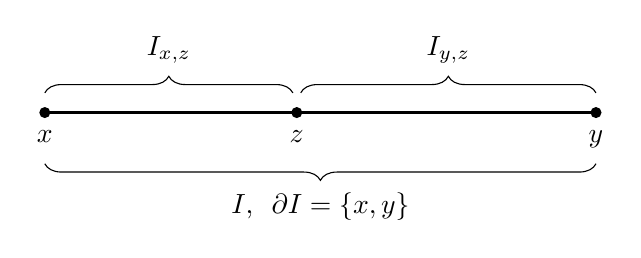
\begin{tikzpicture}[x=1cm,y=1cm]
\draw[line width=1pt] (0,0) -- (7,0);
\foreach \x/\n in {0/x,3.2/z,7/y} { \fill (\x,0) circle (2pt); \node[below] at (\x,-0.1) {$\n$}; }
\draw[decorate, decoration={brace, amplitude=6pt}] (0,0.25) -- (3.15,0.25) node[midway, above=7pt] {$I_{x,z}$};
\draw[decorate, decoration={brace, amplitude=6pt}] (3.25,0.25) -- (7,0.25) node[midway, above=7pt] {$I_{y,z}$};
\draw[decorate, decoration={brace, amplitude=6pt, mirror}] (0,-0.65) -- (7,-0.65) node[midway, below=7pt] {$I$, \ $\partial I = \{x, y\}$};
\end{tikzpicture}
\caption{Axiom F2: for $z$ interior to $I$, the subsegments $I_{x,z}$ and $I_{y,z}$ meet only at $z$. Axiom F4 goes the other way: two segments meeting only at a regular place $z$ glue to a unique segment from $x$ to $y$.}\label{fig:F2}
\end{figure}

Page~10 calls a model a \emph{segment model} when $\cL$ is itself a segment $I_0$, $\partial I_0 = \{x_0, x_1\}$. Page~11 defines $a \le b$ when $a = b$ or $a$ lies on the segment from $x_0$ to $b$, and page~13 concludes that a segment model is the same thing as a \emph{biorder}. Call a partial order \emph{locally directed downwards} if $x < y_1$ and $x < y_2$ imply $x < y \le y_1, y_2$ for some $y$, and \emph{locally directed upwards} in the dual case.

\begin{theorem}[Grothendieck, \fac{156-1}, pp.~10--13]\label{thm:biorder}
In a segment model satisfying F1, F2, F$'$3 and F4, the relation $\le$ is a partial order with least element $x_0$ and greatest element $x_1 \ne x_0$; it is dense and locally directed in both directions; the segments are exactly the intervals $[a, b] = \{z \mid a \le z \le b\}$ with $a < b$, each carried by a single segment; and the order defined from $x_1$ is the opposite order.

Conversely, let $\cL$ be a partially ordered set with distinct least and greatest elements, dense and locally directed in both directions. The intervals $[a, b]$, $a < b$, with $\partial[a, b] = \{a, b\}$, satisfy F1--F5 and F$'$3; $\cL$ is a segment, and the order read from its least element is the given one.
\end{theorem}

\begin{proof}[Sketch]
\emph{Direct sense.} By F1 in $I_0$, a segment is determined by its endpoints (using F2 when neither endpoint is $x_0$ or $x_1$). Transitivity comes from F1 inside $[x_0, c]$; antisymmetry from F2, which forbids $b$ to lie on both sides of an interior point $a$. The key step is \emph{gluing}: if $a$ is regular and a segment $Q$ from $a$ to $z$ meets $[x_0, a]$ only at $a$, then F4 glues them into a segment from $x_0$ to $z$, so $a \le z$. With F2 this shows that the endpoints of every segment are comparable, and that a segment with endpoints $a < b$ is exactly the interval $[a, b]$. Density comes from $I^\circ \ne \emptyset$, the two directedness conditions from F$'$3 at the lower and upper endpoints.

\emph{Converse.} Each axiom becomes a property of intervals: F1 and F2 by the interval structure and density, F$'$3 and F3 by directedness, F4 because two intervals meeting only at $z$ must lie on opposite sides of $z$, and F5 by directedness and density.
\end{proof}

The direct sense uses neither F3 nor F5, and the bounds serve only to make $\cL$ itself a segment. The order need not be total, as the reading of the folder notes.

\begin{example}\label{ex:cone}
On $\Q^2$ let $p \prec q$ when $|q_2 - p_2| < q_1 - p_1$, the order of an open cone, and let $T$ be the set of points between $(0,0)$ and $(2,0)$. It is bounded and dense (the midpoint of $p \prec q$ lies strictly between them), and locally directed both ways: if $x \prec y_1, y_2$, then $x + (\varepsilon, 0)$ works for small $\varepsilon > 0$, and dually $x - (\varepsilon, 0)$. The points $(1, \tfrac12)$ and $(1, -\tfrac12)$ are incomparable (Figure~\ref{fig:cone}). Its intervals therefore form a segment model with a non-total order.
\end{example}

\begin{figure}[ht]
\centering
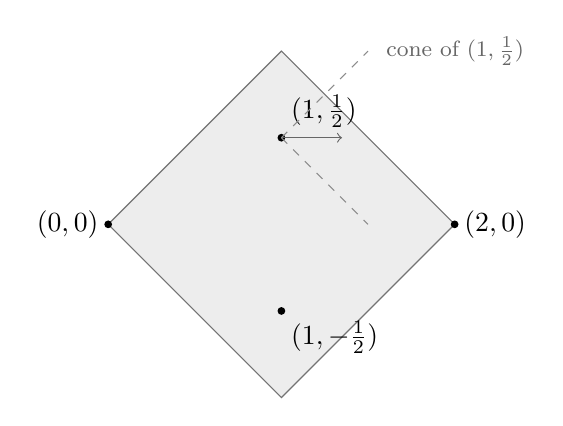
\begin{tikzpicture}[x=2.2cm,y=2.2cm]
\fill[black!7] (0,0) -- (1,1) -- (2,0) -- (1,-1) -- cycle;
\draw[black!55] (0,0) -- (1,1) -- (2,0) -- (1,-1) -- cycle;
\fill (0,0) circle (1.4pt) node[left] {$(0,0)$};
\fill (2,0) circle (1.4pt) node[right] {$(2,0)$};
\fill (1,0.5) circle (1.4pt) node[above right] {$(1,\tfrac12)$};
\fill (1,-0.5) circle (1.4pt) node[below right] {$(1,-\tfrac12)$};
\draw[->,black!60] (1,0.5) -- (1.35,0.5);
\draw[dashed,black!45] (1,0.5) -- (1.5,1) (1,0.5) -- (1.5,0);
\node[black!60,anchor=west] at (1.55,1.0) {\footnotesize cone of $(1,\tfrac12)$};
\end{tikzpicture}
\caption{Example~\ref{ex:cone}: the points between $(0,0)$ and $(2,0)$ for the cone order. Above a point $p$ lie the points of the open cone of half-angle $45^\circ$ opening to the right; $(1, \frac12)$ and $(1, -\frac12)$ are incomparable.}\label{fig:cone}
\end{figure}

\section{The order is read on the cuts}\label{sec:cuts}

Folder~156-3 axiomatises ``networks'' through their cuts. Page~8 defines an \emph{ordered stretch} (\emph{tronçon ordonné}): a partially ordered set, dense, directed upwards and downwards, locally directed in both directions, with more than one element. For comparable $a \ne b$, let $C(\{a, b\})$ be the set of elements distinct from $a$, $b$ and comparable to both; it falls into three \emph{pieces}, the elements below both, strictly between, and above both, and the partition depends only on the pair. Write $X_{\{a,b\}}(t)$ for the piece containing $t$, and $\cR(a, b, c)$ for strict betweenness ($a < b < c$ or $c < b < a$). Page~14 asks whether comparability and the partitions of the $C(\varepsilon)$ into pieces, given without labels, determine $\cR$; page~15 answers ``On gagne !''.

\begin{lemma}[\fac{156-3}, p.~15]\label{lem:pieces}
If $a < b < c$, then $X_{\{a,b\}}(c) = \cL_{>b}$, $X_{\{b,c\}}(a) = \cL_{<b}$ and $X_{\{c,a\}}(b) = \,]a, c[$. If the order is dense and $p, q, r$ are pairwise distinct and comparable, then $\cR(p, q, r)$ holds iff $X_{\{p,q\}}(r) \cap X_{\{q,r\}}(p) = \emptyset$.
\end{lemma}

\begin{proof}
The three pieces are read off the definition. Three pairwise comparable elements form a chain. If $q$ is in the middle, the two pieces are $\cL_{>q}$ and $\cL_{<q}$, which are disjoint. If $p$ is in the middle, say $q < p < r$, they are $\cL_{>p}$ and $]q, r[$, which both contain a point of $]p, r[$, non-empty by density; the other cases are similar.
\end{proof}

\begin{figure}[ht]
\centering
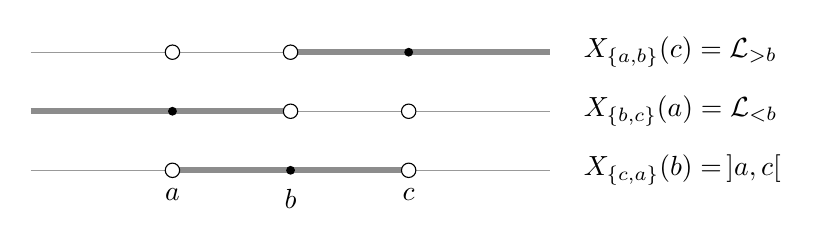
\begin{tikzpicture}[x=1cm,y=0.75cm]
\foreach \row/\p/\q/\lo/\hi/\lab in {0/1.5/3/3/6.3/{$X_{\{a,b\}}(c) = \mathcal L_{>b}$}, -1/3/4.5/-0.3/3/{$X_{\{b,c\}}(a) = \mathcal L_{<b}$}, -2/1.5/4.5/1.5/4.5/{$X_{\{c,a\}}(b) = \,]a,c[$}} {
  \draw[black!40] (-0.3,\row) -- (6.3,\row);
  \draw[line width=2.2pt, black!45] (\lo,\row) -- (\hi,\row);
  \foreach \x in {1.5,3,4.5} \fill (\x,\row) circle (1.6pt);
  \draw[fill=white] (\p,\row) circle (2.6pt);
  \draw[fill=white] (\q,\row) circle (2.6pt);
  \node[anchor=west] at (6.6,\row) {\lab};
}
\foreach \x/\n in {1.5/a,3/b,4.5/c} \node[below] at (\x,-2.15) {$\n$};
\end{tikzpicture}
\caption{Lemma~\ref{lem:pieces} on a chain $a < b < c$: each pair (white circles, excluded from $C(\varepsilon)$) cuts the rest into three pieces; the thick part is the piece containing the third point. The first two thick pieces are disjoint: $b$ is between $a$ and $c$.}\label{fig:cuts}
\end{figure}

\begin{theorem}[after \fac{156-3}, pp.~11--15]\label{thm:cuts}
A bijection between two ordered stretches that respects comparability and, for every comparable pair $\varepsilon$, the partition of $C(\varepsilon)$ into pieces, is an order isomorphism or an anti-isomorphism. Comparability alone does not suffice: on the stretch $\Q$, the transposition of $0$ and $1$ respects comparability and is neither increasing nor decreasing.
\end{theorem}

\begin{proof}
By Lemma~\ref{lem:pieces} the bijection respects strict betweenness. Pages~11--13 show that betweenness and comparability determine the order up to reversal: for $a < b$, one has $u \le v$ iff there are $x$ and $y$, with $x = a$ or $\cR(b, a, x)$ and $y = b$ or $\cR(a, b, y)$, such that $x \le u \le y$, $x \le v \le y$ and $u$ lies weakly between $x$ and $v$; the conditions are expressed by betweenness alone once the large form ``$\cR(a, b, c)$, or $b \in \{a, c\}$ with $a$ and $c$ comparable'' is used, and directedness supplies $x$ and $y$. Transporting this description along the bijection, with the opposite order on the target if $e(b) < e(a)$, gives the result. For $\Q$, $\sigma(1) = 0 < 1 = \sigma(0)$ while $\sigma(1) = 0 < 2 = \sigma(2)$.
\end{proof}

Only density and two-sided directedness are used, so the theorem holds for every dense partial order directed in both directions. The second sentence is ours. The large form of betweenness needs the comparability clause: the reading's form ``$\cR(a, b, c)$ or $b \in \{a, c\}$'' fails for incomparable $a$, $c$, for instance in $\mathbb N^2$ with the product order. The reconstruction of a partial order up to reversal from its strict betweenness is studied by Courcelle \cite[\S1, Th.~7]{courcelle2020}.

\section{Sides of a subset}\label{sec:sides}

Folder~156-2 cuts a space along a closed subset without assuming a manifold or a triangulation. For $A \subseteq X$, $j\colon X \setminus A \hookrightarrow X$, and $\mathrm{Comp}(Z)$ the Boolean ring of clopen subsets of $Z$, page~14 puts
\[
\mathrm{Riv}(A, X) = \varinjlim_{V \supseteq A} \mathrm{Comp}(V \setminus A),
\]
the \emph{sides} of $A$, the limit over neighbourhoods of $A$, and $\widetilde A = \operatorname{Spec}(j_*\mathbb F_2)$. Page~15 writes a canonical map $\mathrm{Riv}(A, X) \to \mathrm{Comp}(\widetilde A)$, ``injective'', with ``bijective if $X$ is paracompact'' added above the line. We take for $\widetilde A$ the set of pairs $(x, \chi)$, $x \in A$, $\chi$ a point of the spectrum of the stalk of $j_*\mathbb F_2$ at $x$, with the topology generated by the sets where a locally constant function on $W \setminus A$ takes the value $1$.

\begin{theorem}[after \fac{156-2}, pp.~14--15]\label{thm:sides}
For every subset $A$ of every topological space $X$, the image of each side is clopen in $\widetilde A$, the map $\mathrm{Riv}(A, X) \to \mathrm{Comp}(\widetilde A)$ is a morphism of Boolean algebras, and it is injective. The ring $\mathrm{Riv}(A, X)$ is zero iff $A$ is open.
\end{theorem}

\begin{proof}[Sketch]
Two distinct germs at $x$ are separated by a point of the spectrum of the stalk, obtained as evaluation along an ultrafilter finer than the filter of neighbourhoods of $x$ in $X \setminus A$. The other statements are formal.
\end{proof}

Closedness of $A$ is not used. The last statement corrects ``$A \ne \emptyset$'' in the remark on bi-sides to ``$A$ not open''. Bijectivity for paracompact $X$ is not proved here.

\section{Saturated parts are not a Boolean algebra}\label{sec:sat}

Folder~156-4 starts from a stratified space and abstracts a partially ordered set $(\cM, \le)$ of \emph{multistrata} with a symmetric relation $R$, \emph{compatibility}, reflexive and inherited downwards. On pages~65--68, two multistrata are \emph{disjoint} if they are compatible and have no common lower bound; the \emph{cosupport} $\Phi'$ of $\Phi \subseteq \cM$ is the set of multistrata disjoint from every element of $\Phi$, the \emph{support} is $\Phi''$, and $\Phi$ is \emph{saturated} if $\Phi = \Phi''$. Page~68 guesses that the saturated parts form a Boolean algebra, even ``ultra-Stonean''.

\begin{proposition}[after \fac{156-4}, pp.~66--67]\label{prop:ortho}
For any partially ordered set $(\cM, \le)$ with a symmetric relation $R$, intersections of saturated parts are saturated, every cosupport is saturated, and on saturated parts the cosupport is an inclusion-reversing involution with $S \cap S' = \emptyset$ and $(S \cup S')'' = \cM$. The saturated parts form a complete orthocomplemented lattice.
\end{proposition}

This is the classical lattice of closed sets of a polarity: for orthogonality in a Euclidean space, the closed sets are the subspaces, which do not form a Boolean algebra. The axioms of the folder do not exclude this phenomenon.

\begin{theorem}[after \fac{156-4}, p.~68]\label{thm:hexagon}
Let $\cM$ have four minimal elements $a, b, c, d$ and three elements $v_{ab}$, $v_{bc}$, $v_{cd}$, each above the pair it indexes, and let compatibility be generated by the pairs lying under a common $v$. Then $\le$ is an order, $R$ is reflexive, symmetric and inherited downwards, and the saturated parts are exactly
\[
\emptyset,\quad \{b\},\quad \{c\},\quad \{a, c\},\quad \{b, d\},\quad \cM.
\]
They form a hexagon, which is not distributive: $\{b, d\} \wedge (\{b\} \vee \{c\}) = \{b, d\}$, while $(\{b, d\} \wedge \{b\}) \vee (\{b, d\} \wedge \{c\}) = \{b\}$.
\end{theorem}

\begin{proof}
The disjoint pairs are $\{a, b\}$, $\{b, c\}$, $\{c, d\}$, so the cosupport of a part is the set of common neighbours of its elements in the path $a - b - c - d$. Thus $\{b\}' = \{a, c\}$, $\{a, c\}' = \{b\}$, $\{c\}' = \{b, d\}$, $\{b, d\}' = \{c\}$ and $\{b, c\}' = \emptyset$; the list is checked on all $128$ parts. The join of $\{b\}$ and $\{c\}$ is $\{b, c\}'' = \cM$.
\end{proof}

\begin{figure}[ht]
\centering
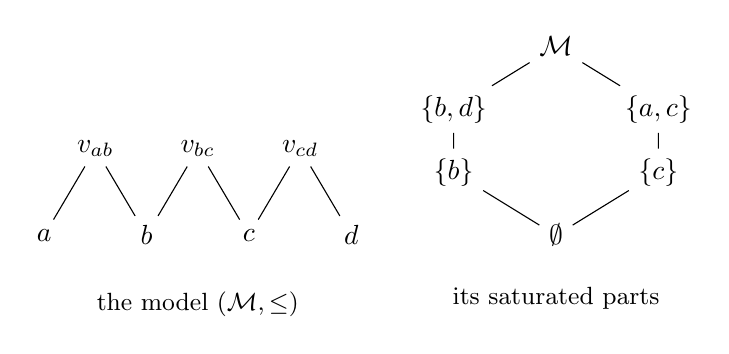
\begin{tikzpicture}[x=1.3cm,y=1.1cm]
\begin{scope}
\foreach \n/\x in {a/0,b/1,c/2,d/3} \node (\n) at (\x,0) {$\n$};
\node (vab) at (0.5,1) {$v_{ab}$}; \node (vbc) at (1.5,1) {$v_{bc}$}; \node (vcd) at (2.5,1) {$v_{cd}$};
\draw (a) -- (vab) -- (b) -- (vbc) -- (c) -- (vcd) -- (d);
\node at (1.5,-0.8) {\small the model $(\mathcal M, \le)$};
\end{scope}
\begin{scope}[xshift=6.5cm, y=0.8cm]
\node (bot) at (0,0) {$\emptyset$};
\node (b) at (-1,1) {$\{b\}$}; \node (bd) at (-1,2) {$\{b,d\}$};
\node (c) at (1,1) {$\{c\}$}; \node (ac) at (1,2) {$\{a,c\}$};
\node (top) at (0,3) {$\mathcal M$};
\draw (bot) -- (b) -- (bd) -- (top) -- (ac) -- (c) -- (bot);
\node at (0,-1) {\small its saturated parts};
\end{scope}
\end{tikzpicture}
\caption{Theorem~\ref{thm:hexagon}: the seven-element model and the hexagon lattice of its saturated parts, which is orthocomplemented ($\{b\} \leftrightarrow \{a,c\}$, $\{c\} \leftrightarrow \{b,d\}$) but not distributive.}\label{fig:hexagon}
\end{figure}

Whether the later disjointness axioms of the folder (C\,5, page~69, and the ``packet of disjointness axioms'' of page~85) restore distributivity is not decided here. When $R$ is always true, the saturated parts are the regular open sets of $(\cM, \le)$ and do form a complete Boolean algebra.

\section{Coarsest cell decompositions in a tame Boolean algebra}\label{sec:tame}

Folder~121, \emph{Topologie modérée}, looks for a notion of tame subset of a topological space $X$. Pages~3--5 take a Boolean algebra $\mathcal F$ of subsets of $X$ and the conditions: (c~bis) $A \in \mathcal F \Rightarrow \overline A \in \mathcal F$; (d) every $A \in \mathcal F$ contains a dense open subset of its closure, open relative to the closure; (e) every decreasing sequence of closed members of $\mathcal F$, each nowhere dense in the previous one, reaches $\emptyset$. Page~8 shows that the frontier of a member is nowhere dense. Page~10 calls a \emph{cell decomposition} a finite partition of $X$ such that the closure of each cell is a union of cells and distinct cells have distinct closures; it is \emph{$\mathcal F$-admissible} if its cells are in $\mathcal F$.

\begin{theorem}[Grothendieck, \fac{121}, pp.~14 and~16]\label{thm:cells}
Let $\mathcal F$ satisfy (c~bis), (d) and (e). Every finite family $\mathcal L \subseteq \mathcal F$ has an $\mathcal F$-admissible cell decomposition in which each member of $\mathcal L$ is a union of cells, and among these a coarsest one. If moreover (f) for closed $B, C \in \mathcal F$ the connected components of $B \setminus C$ are finite in number and belong to $\mathcal F$, the same holds for decompositions with connected cells.
\end{theorem}

\begin{proof}[Sketch]
Following page~14, induct on a closed member $Z$ in place of $X$: remove the union of the frontiers, relative to $Z$, of the members of the family and of their closures, which is nowhere dense by page~8, and stop by (e). The cells are the non-empty patterns of membership on the open part, and the decomposition of the removed closed part. Page~14 asserts without argument that the result is the coarsest. Our argument: a cell of any decomposition in which $Y$ is a union of cells and which meets the frontier of $Y$ is contained in it, so every admissible decomposition restricts to the removed part and refines the open cells. For connected cells (page~16), replace the open cells by their connected components, which (f) controls since an open cell is $\overline U \setminus X'$; a connected cell of a competing decomposition inside $U$ lies in one component.
\end{proof}

Figure~\ref{fig:cells} shows the result on a closed disc.

\begin{figure}[ht]
\centering
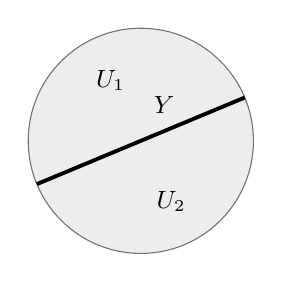
\begin{tikzpicture}[scale=1.1]
\fill[black!7] (0,0) circle (1.3);
\draw[black!55] (0,0) circle (1.3);
\draw[line width=1.4pt] (-1.2,-0.5) -- (1.2,0.5);
\node at (-0.35,0.7) {\small $U_1$};
\node at (0.35,-0.7) {\small $U_2$};
\node[above left] at (0.5,0.2) {\small $Y$};
\end{tikzpicture}
\caption{Theorem~\ref{thm:cells} with connected cells, for $X$ a closed disc, $\mathcal F$ its semialgebraic subsets and $\mathcal L = \{Y\}$, $Y$ a closed chord from boundary to boundary. Removing the frontier of $Y$, which is $Y$ itself, leaves an open set with two components $U_1$, $U_2$; the coarsest decomposition with connected cells is $\{U_1, U_2, Y\}$, and $\overline{U_i} = U_i \cup Y$.}\label{fig:cells}
\end{figure}

\section{Verification}\label{sec:lean}
\begingroup\sloppy
Every theorem above is formalised in Lean~4 with Mathlib, in the files \nolinkurl{Folder156_1.lean} (\nolinkurl{biorder}, \nolinkurl{intervals_segModel}, \nolinkurl{not_total}), \nolinkurl{Folder156_3.lean} (\nolinkurl{middle_iff}, \nolinkurl{order_eq_or_dual}, \nolinkurl{order_of_cuts}, \nolinkurl{cmp_alone_insufficient}), \nolinkurl{Folder156_2.lean} (\nolinkurl{toComp_injective}, \nolinkurl{toComp_mul}, \nolinkurl{riv_one_eq_zero_iff}), \nolinkurl{Folder156_4.lean} (\nolinkurl{cosupp_cosupp}, \nolinkurl{supp_union_cosupp}, \nolinkurl{hexagon_saturated}, \nolinkurl{hexagon_not_distrib}) and \nolinkurl{Folder121.lean} (\nolinkurl{page14}, \nolinkurl{page16}) of the repository \href{https://github.com/Commutator-IO/grothendieck-project}{Commutator-IO/grothendieck-project}, using only Lean's standard axioms. Not proved here: the corollaries of F1, F2, F4 outside segment models, restriction and orientation (folder~156-1, pp.~8--17); the bijectivity of Theorem~\ref{thm:sides} for paracompact spaces and the cut space of pages~16--17; the axioms of networks by cuts (folder~156-3, pp.~1--5 and~16--39); the later disjointness axioms of folder~156-4; the regular decompositions of folder~121, page~17.
\endgroup

\section*{Statement on the use of artificial intelligence}
The transcriptions of the folders, the modernised readings, the proofs, the Lean formalisation and a first draft of this text were produced with language models (Claude Opus~5 and Opus~5.5, Anthropic), under the author's direction. The author checked the statements, the proofs and the references, and takes full responsibility for the content. The formal proofs are checked mechanically by Lean.

\section*{Acknowledgements}
The facsimiles are published by the University of Montpellier, \href{https://grothendieck.umontpellier.fr/}{grothendieck.umontpellier.fr}.

\begin{thebibliography}{9}
\bibitem{courcelle2020} B.~Courcelle, Betweenness of partial orders, \emph{RAIRO Theor.\ Inform.\ Appl.} 54 (2020), article~7, \href{https://doi.org/10.1051/ita/2020007}{doi:10.1051/ita/2020007}.
\bibitem{esquisse} A.~Grothendieck, Esquisse d'un programme, in L.~Schneps, P.~Lochak (eds.), \emph{Geometric Galois Actions 1}, London Math.\ Soc.\ Lecture Note Ser.~242, Cambridge University Press, 1997, 7--48, \href{https://doi.org/10.1017/CBO9780511758874.003}{doi:10.1017/CBO9780511758874.003}.
\bibitem{vandendries1998} L.~van den Dries, \emph{Tame Topology and O-minimal Structures}, London Math.\ Soc.\ Lecture Note Ser.~248, Cambridge University Press, 1998, \href{https://doi.org/10.1017/CBO9780511525919}{doi:10.1017/CBO9780511525919}.
\end{thebibliography}

\end{document}
